\documentclass[../main/main.tex]{subfiles}

\newdate{date}{25}{11}{2020}

% \begin{figure}[h!]
% \centering
% \includegraphics[page=6,width=0.8\textwidth]{../lessons/pdf_file/20_lecture.pdf}
% \end{figure}

%\displaydate{date}. Compiled:  \today. Alice.

\begin{document}

\pagestyle{plain}

\section{Lecture 20}


\subsubsection*{Slide 1}

\begin{minipage}[]{0.5\linewidth}
\centering
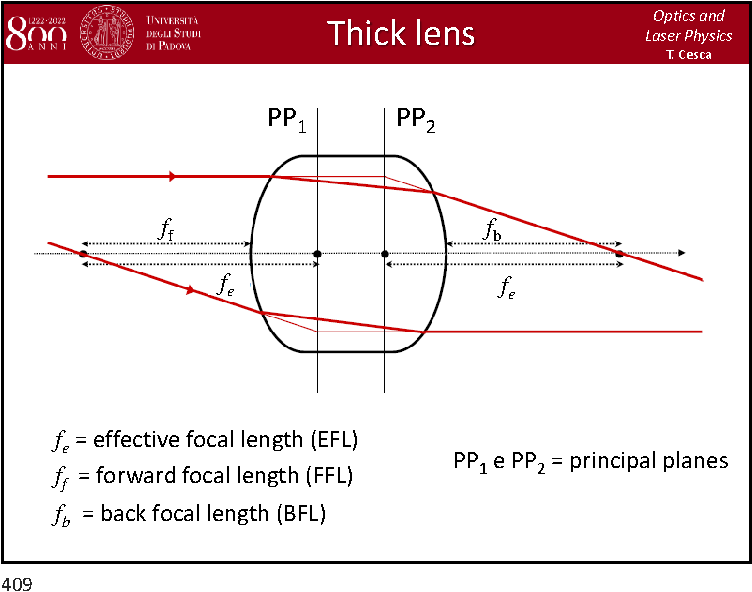
\includegraphics[page=1,width=1\textwidth]{../lessons/pdf_file/20_lecture.pdf}
\end{minipage}
\hspace{0.3cm}\vspace{0.3cm}
\begin{minipage}[c]{0.47\linewidth}

Let us apply the ABCD matrix approach for a \textbf{thick lens}. The thickness cannot be neglected. One important result we can no longer introduce just one focal length, but we have to associate to the lens three difference focal lens: EFL, FFL, BFL.

The \textbf{effective focal length} is the equivalent of the focal length for the thin lens provided that the distance of the image is calculated by the so called \textbf{principale planes}.

At the distance of FFL, with a point source here we obtain a collimated beam (a beam which is parallel to the optical axis outside of the lens).

The same idea for BFL, a collimated beam will be converged to the focal point BFL.

\end{minipage}

\subsubsection*{Slide 2}

\begin{minipage}[]{0.5\linewidth}
\centering
\includegraphics[page=2,width=1\textwidth]{../lessons/pdf_file/20_lecture.pdf}
\end{minipage}
\hspace{0.3cm}\vspace{0.3cm}
\begin{minipage}[c]{0.47\linewidth}

Let us consider the most general situation with two dipters with two different radii of curvature.

If the lens is not in air, \( n \) is the refractive index of the lens wrt the refractive index of the medium in which the lens is embedded.

\end{minipage}

\subsubsection*{Slide 3}

\begin{minipage}[]{0.5\linewidth}
\centering
\includegraphics[page=3,width=1\textwidth]{../lessons/pdf_file/20_lecture.pdf}
\end{minipage}
\hspace{0.3cm}\vspace{0.3cm}
\begin{minipage}[c]{0.47\linewidth}

We can define the effective focal length. So, it is given by the entries \( C \).

We are not demostrating these results!

\end{minipage}

\newpage

\subsubsection*{Slide 4}

\begin{minipage}[]{0.5\linewidth}
\centering
\includegraphics[page=4,width=1\textwidth]{../lessons/pdf_file/20_lecture.pdf}
\end{minipage}
\hspace{0.3cm}\vspace{0.3cm}
\begin{minipage}[c]{0.47\linewidth}

We can now write an expression formally equivalent to the thin lens equation provided that the distances of the object and of the image are measured from the corresponding principal planes.
So, you can apply for instance ray tracing if you compute the distances from the principale planes.

\end{minipage}

\subsubsection*{Slide 5}

\begin{minipage}[]{0.5\linewidth}
\centering
\includegraphics[page=5,width=1\textwidth]{../lessons/pdf_file/20_lecture.pdf}
\end{minipage}
\hspace{0.3cm}\vspace{0.3cm}
\begin{minipage}[c]{0.47\linewidth}

The thick lens is a peculiar optical system: two spherical diopters with propagation in free-space inside.

Any optical system can be treated as we did for the thick lens. Any optical system can be considered as a black box, its needed only to the determine the most important parameters which are FFL, BFL and also principal planes.

\end{minipage}

\subsubsection*{Slide 6}

\begin{minipage}[]{0.5\linewidth}
\centering
\includegraphics[page=6,width=1\textwidth]{../lessons/pdf_file/20_lecture.pdf}
\end{minipage}
\hspace{0.3cm}\vspace{0.3cm}
\begin{minipage}[c]{0.47\linewidth}

Let us consider a generic optical system composed by two lenses at a distance \( d \) (or it can be even more complicated). The idea is that when you calculate the effective focal length you have an equation similar to the one of thin lenses.

Once you have determine \( p \) and \( q \), you can compute the \textbf{magnification}.

\end{minipage}

\newpage

\subsubsection*{Slide 7}

\begin{minipage}[]{0.5\linewidth}
\centering
\includegraphics[page=7,width=1\textwidth]{../lessons/pdf_file/20_lecture.pdf}
\end{minipage}
\hspace{0.3cm}\vspace{0.3cm}
\begin{minipage}[c]{0.47\linewidth}

You can calculate the position of the principal planes: the \textbf{forward principal plane} \( h_f \) and the \textbf{backward principal plane} \( h_b \).

We should note the minus sign \( h_b \) which is due to the fact that the principal planes on the left of the corresponding lens have negative distance.

Positive distance for \( h_f \) and \( h_b \), it means that the principal plane is on the right of the corresponding optical element.

If you get negative distance, it means that the principal plane is on the left.

\end{minipage}

\subsubsection*{Slide 8}

\begin{minipage}[]{0.5\linewidth}
\centering
\includegraphics[page=8,width=1\textwidth]{../lessons/pdf_file/20_lecture.pdf}
\end{minipage}
\hspace{0.3cm}\vspace{0.3cm}
\begin{minipage}[c]{0.47\linewidth}

Let us make an exercise.
We are considering thin lens.

\end{minipage}

\subsubsection*{Slide 9}

\begin{minipage}[]{0.5\linewidth}
\centering
\includegraphics[page=9,width=1\textwidth]{../lessons/pdf_file/20_lecture.pdf}
\end{minipage}
\hspace{0.3cm}\vspace{0.3cm}
\begin{minipage}[c]{0.47\linewidth}


\end{minipage}

\subsubsection*{Slide 10}

\begin{minipage}[]{0.5\linewidth}
\centering
\includegraphics[page=10,width=1\textwidth]{../lessons/pdf_file/20_lecture.pdf}
\end{minipage}
\hspace{0.3cm}\vspace{0.3cm}
\begin{minipage}[c]{0.47\linewidth}

Pay attention to the sign of the quantities!

We are realizing a \textbf{beam expander}: we have a double height.

\end{minipage}

\subsubsection*{Slide 11}

\begin{minipage}[]{0.5\linewidth}
\centering
\includegraphics[page=11,width=1\textwidth]{../lessons/pdf_file/20_lecture.pdf}
\end{minipage}
\hspace{0.3cm}\vspace{0.3cm}
\begin{minipage}[c]{0.47\linewidth}

We can think it in this way.

If we look at it from left to right we have a beam expander, but if we look at it from right to left we have a \textbf{Galilean telescope}.

In the Keplerian telescope we have two convergence focal lens.

\end{minipage}

\subsubsection*{Slide 12}

\begin{minipage}[]{0.5\linewidth}
\centering
\includegraphics[page=12,width=1\textwidth]{../lessons/pdf_file/20_lecture.pdf}
\end{minipage}
\hspace{0.3cm}\vspace{0.3cm}
\begin{minipage}[c]{0.47\linewidth}

Let us make another exercise.

\( p \) and \( q \) are the distances from the corresponding principal planes!

\end{minipage}

\subsubsection*{Slide 13}

\begin{minipage}[]{0.5\linewidth}
\centering
\includegraphics[page=13,width=1\textwidth]{../lessons/pdf_file/20_lecture.pdf}
\end{minipage}
\hspace{0.3cm}\vspace{0.3cm}
\begin{minipage}[c]{0.47\linewidth}

Remember that the paramaters have a given sign!

\end{minipage}

\subsubsection*{Slide 14}

\begin{minipage}[]{0.5\linewidth}
\centering
\includegraphics[page=14,width=1\textwidth]{../lessons/pdf_file/20_lecture.pdf}
\end{minipage}
\hspace{0.3cm}\vspace{0.3cm}
\begin{minipage}[c]{0.47\linewidth}

In this case the distances are both positive, it means that they are both on the right of the corresponding optical elements!

Positive \( h_f \) on the right of the first lens, positve \( h_b \) on the right of the second optical element! The distance is referred to the distance of the corresponding optical element!
They can be in any position.


\end{minipage}

\subsubsection*{Slide 15}

\begin{minipage}[]{0.5\linewidth}
\centering
\includegraphics[page=15,width=1\textwidth]{../lessons/pdf_file/20_lecture.pdf}
\centering
\includegraphics[page=16,width=1\textwidth]{../lessons/pdf_file/20_lecture.pdf}
\end{minipage}
\hspace{0.3cm}\vspace{0.3cm}
\begin{minipage}[c]{0.47\linewidth}

Let us determine the transverse magnification.

The image that you form has exactly the same size of the object. The object does not change the dimension.


\end{minipage}



\end{document}
